\documentclass[11pt,a4paper]{article}

\usepackage[a4paper,margin=1in]{geometry}
\usepackage{graphicx}
\usepackage{booktabs}
\usepackage{amsmath,amssymb}
\usepackage{float}
\usepackage{hyperref}
\usepackage{xcolor}
\usepackage{listings}
\usepackage{enumitem}
\usepackage{fancyhdr}
\usepackage{longtable}
\usepackage{array}

\hypersetup{colorlinks=true,linkcolor=blue,urlcolor=blue}

\pagestyle{fancy}
\setlength{\headheight}{14pt}
\fancyhf{}
\lhead{Computer Networks Laboratory}
\rhead{Assignment 1}
\cfoot{\thepage}

\lstdefinestyle{cstyle}{
  language=C,
  basicstyle=\ttfamily\small,
  numbers=left,
  numberstyle=\tiny,
  frame=single,
  breaklines=true,
  showstringspaces=false,
  keywordstyle=\color{blue},
  commentstyle=\color{gray},
  stringstyle=\color{purple}
}
\lstset{style=cstyle}

\begin{document}

\begin{tabular}{|p{4cm}|p{11cm}|}
\hline
Assignment No. & 1 \\ \hline
Title & Study of Networking Diagnostic \& Monitoring Tools and Socket Programming System Calls\footnotemark \\ \hline
Student Name & Simiyon Vinscent Samuel L \\ \hline
Register Number & 3122247001062 \\ \hline
Submission Date & August 17, 2026 \\ \hline
\end{tabular}
\footnotetext{\textbf{GitHub Repository: }\url{https://github.com/blackscythe123/PCN-assign}}

\section{Aim}
To apply and analyse standard Linux networking diagnostic and monitoring tools in order to
observe network status, interface configuration, connectivity, routing and performance
(Part A), and to study the socket-programming system calls that these tools are themselves
built on top of, so that their behaviour at the API level is understood well enough to be
reproduced in a C program (Part B).

\section{Environment}
\begin{tabular}{ll}
\toprule
Operating System & Ubuntu (WSL2) on Windows 11 \\
Kernel networking & WSL2 virtual NAT adapter (\texttt{eth0}) \\
Shell & bash 5.x \\
Compiler & gcc (Part B) \\
Hostname used in captures & \texttt{samsamuel} \\
\bottomrule
\end{tabular}

All commands below were executed for real in a WSL2 Ubuntu terminal. Every figure is an
unedited screenshot of that terminal; the exact text output is also archived under
\texttt{as1/logs/} in the repository for cross-checking, and the socket-programming source
used in Part B is under \texttt{as1/src/}.

\clearpage
\section{Part A --- Networking Diagnostic \& Monitoring Tools}

%===================================================================
\subsection{netstat}
\textbf{Purpose:} Displays active network connections, listening ports, and (with \texttt{-p},
as root) the owning process for each socket.\\
\textbf{Command used:} \texttt{netstat -tulnp}

\begin{figure}[H]
\centering
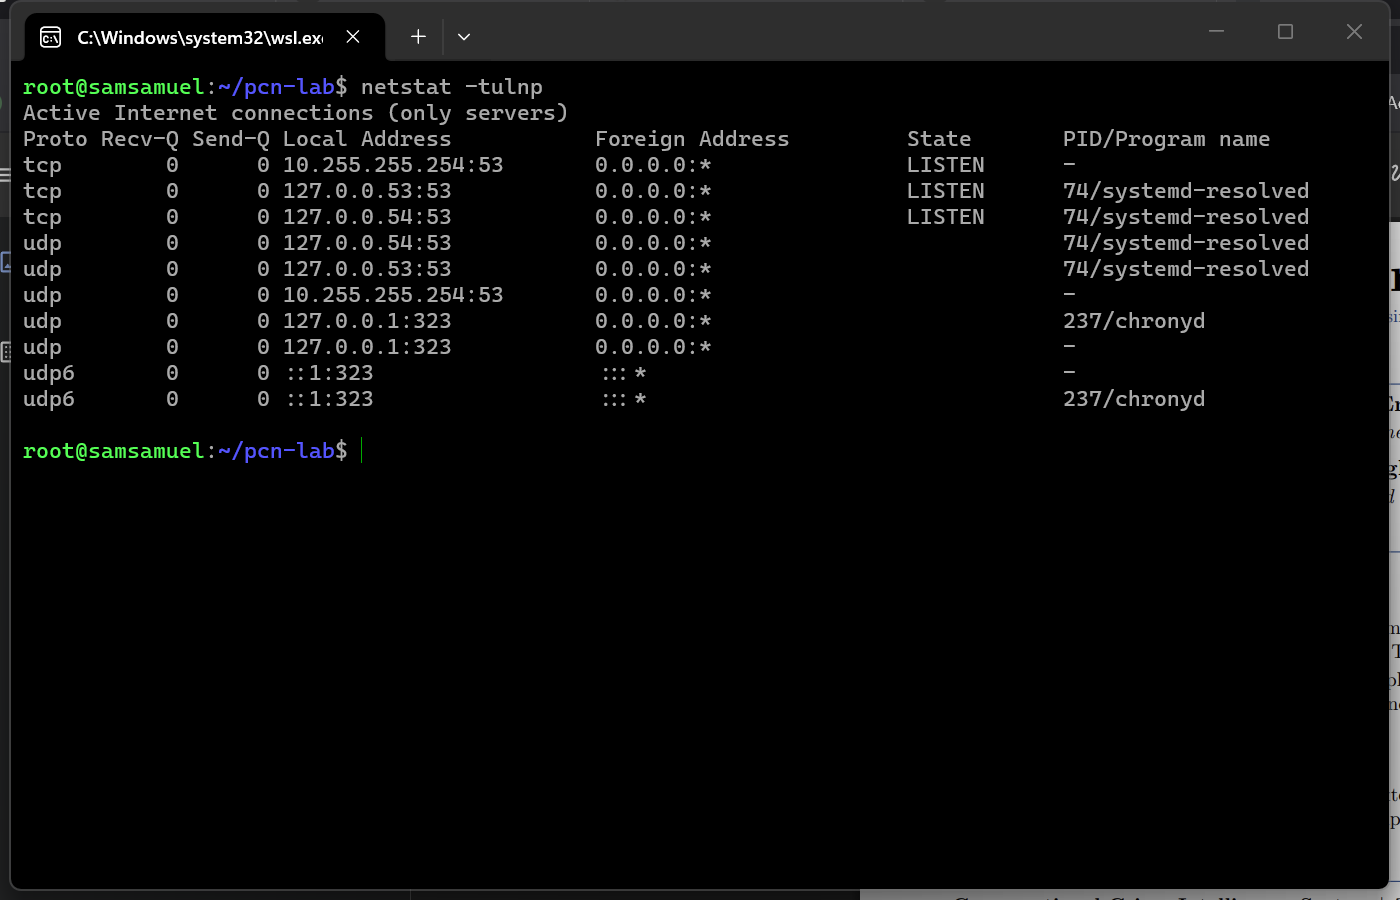
\includegraphics[width=0.85\linewidth]{ss/01_netstat.png}
\caption{netstat -tulnp -- TCP/UDP listening sockets}
\end{figure}

\textbf{Observation:} The only services listening in this WSL instance are
\texttt{systemd-resolved} (Ubuntu's local DNS stub resolver, bound to \texttt{127.0.0.53:53},
\texttt{127.0.0.54:53} and the WSL-internal \texttt{10.255.255.254:53} on both TCP and UDP)
and \texttt{chronyd}, the NTP client, bound to UDP port 323 on IPv4 and IPv6 loopback. No
externally reachable service is listening, which is expected for a bare lab VM that has not
been configured as a server yet -- this baseline is useful to compare against once
Assignment 2/3's TCP/UDP servers are started, since their listening sockets should then also
show up here.

%===================================================================
\subsection{ifconfig}
\textbf{Purpose:} Displays and can configure network interface parameters -- IP address,
netmask, broadcast address, MTU, and interface statistics (packets/bytes sent and received).\\
\textbf{Command used:} \texttt{ifconfig}

\begin{figure}[H]
\centering
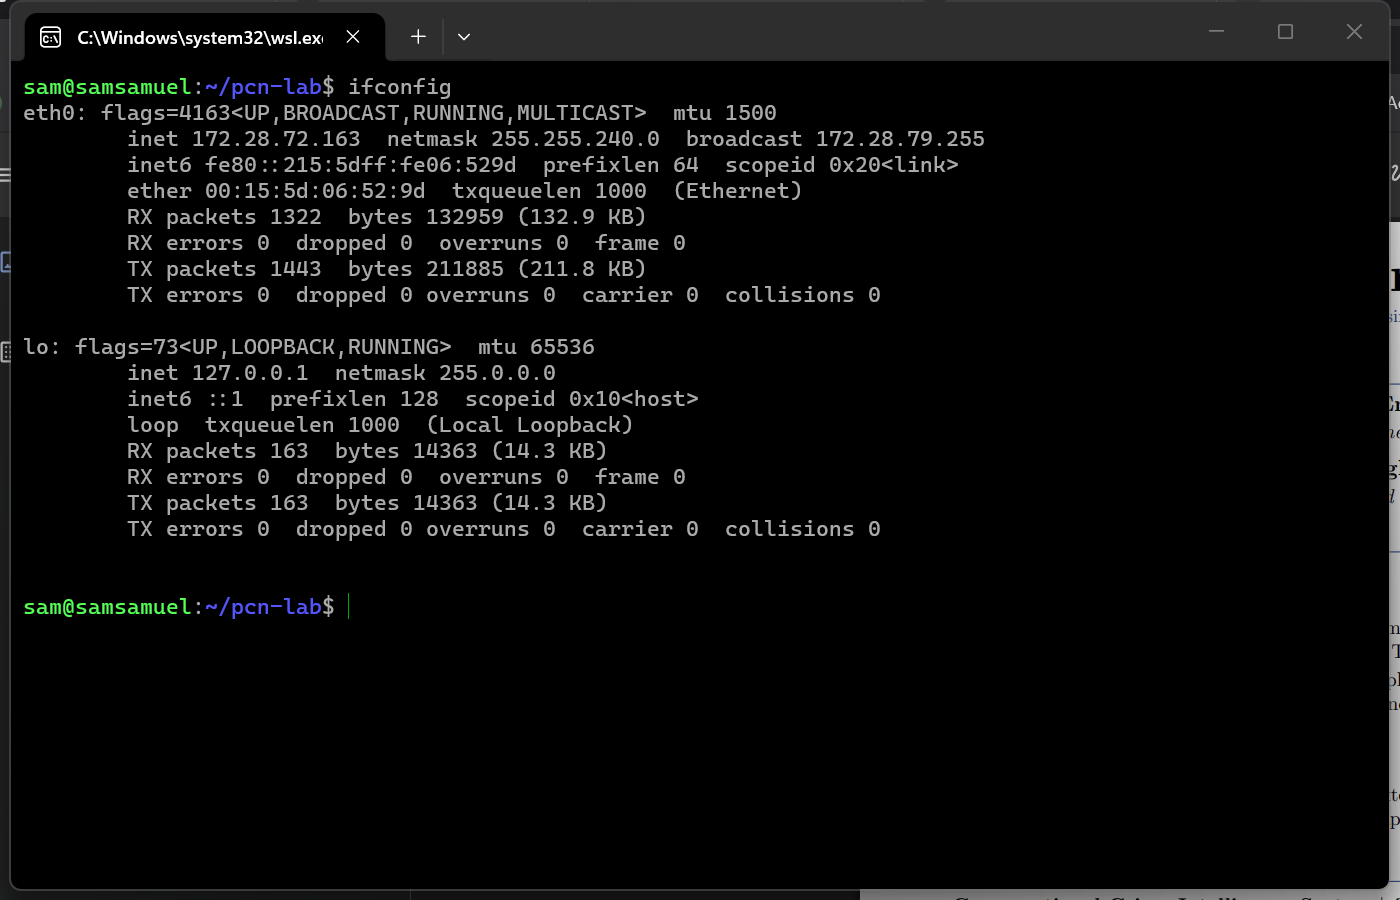
\includegraphics[width=0.85\linewidth]{ss/02_ifconfig.png}
\caption{ifconfig -- interface configuration}
\end{figure}

\textbf{Observation:} \texttt{eth0} is the single virtual NIC that WSL2 presents to Ubuntu,
with address \texttt{172.28.72.163/20} (netmask \texttt{255.255.240.0}, broadcast
\texttt{172.28.79.255}), MAC \texttt{00:15:5d:06:52:9d} and MTU 1500. This is a
Hyper-V-backed adapter NAT'ed behind the Windows host, which is why the address is in a
private \texttt{172.28.0.0/20} range rather than the host machine's real LAN. \texttt{lo}
(loopback, \texttt{127.0.0.1/8}) shows matching RX/TX byte counts, confirming every packet
sent to loopback is received back locally with nothing dropped.

%===================================================================
\subsection{iwconfig}
\textbf{Purpose:} Displays and configures wireless-specific interface parameters -- SSID,
frequency/channel, transmit power, link quality and signal strength -- the wireless
counterpart to \texttt{ifconfig}.\\
\textbf{Command used:} \texttt{iwconfig} (attempted)

\textbf{Observation:} \texttt{iwconfig} could not be demonstrated in this environment. It
ships in the \texttt{wireless-tools} package, which is no longer available in this Ubuntu
release's repositories (superseded by the newer \texttt{iw} utility upstream). More
fundamentally, WSL2 only exposes a single virtual, wired NAT adapter (\texttt{eth0}, seen in
Section~2.2) -- there is no wireless hardware in the VM for \texttt{iwconfig} to report on,
so even if the legacy package were installed it would only print
\texttt{eth0 \ no wireless extensions.} for every interface. On a physical Linux machine with
a Wi-Fi card, \texttt{iwconfig wlan0} would instead show fields such as \texttt{ESSID},
\texttt{Frequency}, \texttt{Access Point}, \texttt{Bit Rate}, \texttt{Link Quality} and
\texttt{Signal level}.

%===================================================================
\subsection{ping}
\textbf{Purpose:} Sends ICMP Echo Request packets to a destination and reports Echo Reply
round-trip time, used to verify basic reachability and measure latency/packet loss.\\
\textbf{Command used:} \texttt{ping -c 4 8.8.8.8}

\begin{figure}[H]
\centering
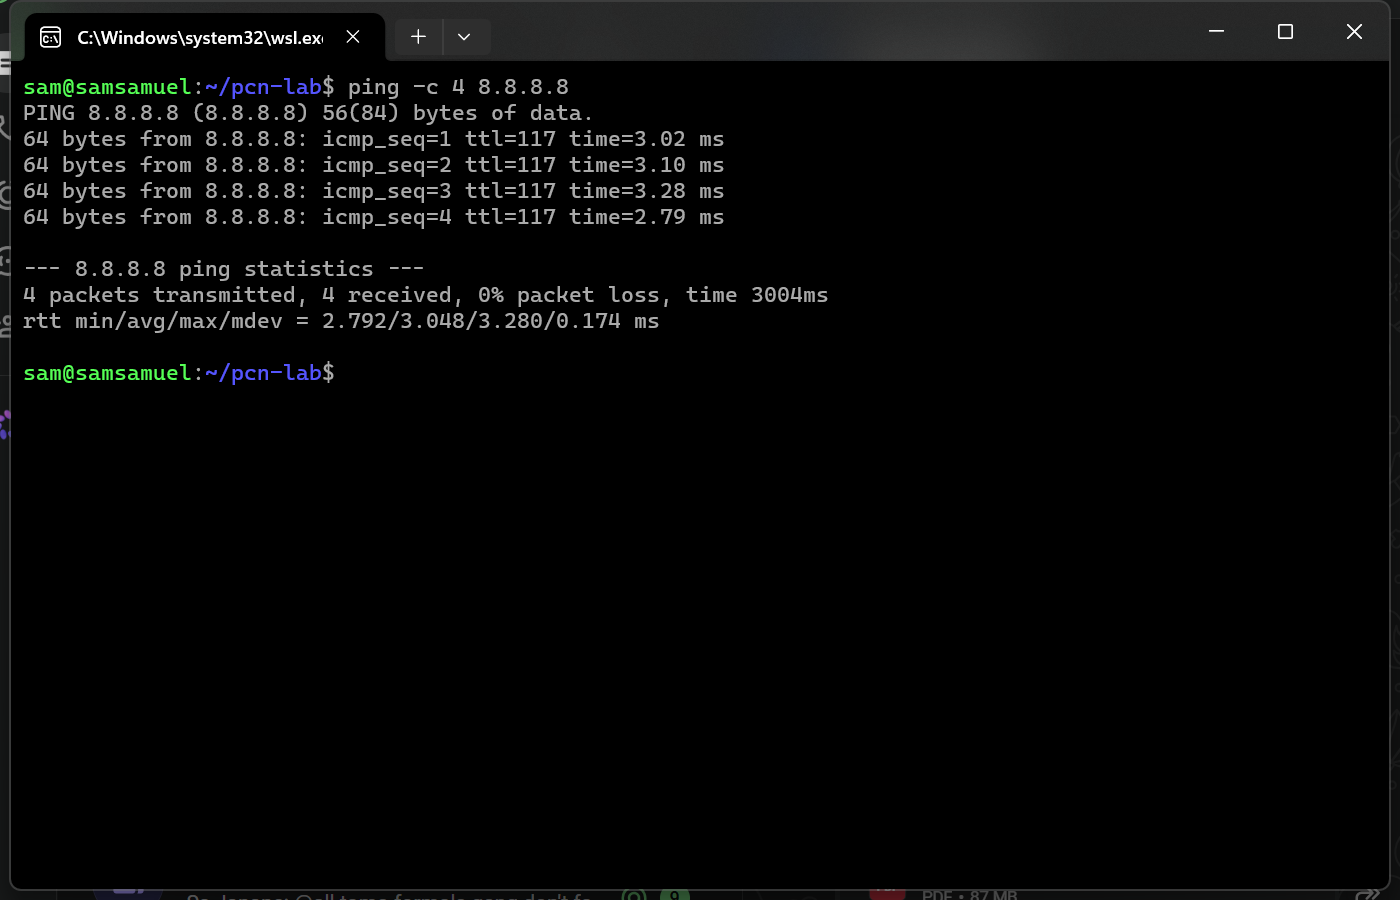
\includegraphics[width=0.85\linewidth]{ss/04_ping.png}
\caption{ping -c 4 8.8.8.8}
\end{figure}

\textbf{Observation:} All 4 ICMP packets sent to Google's public DNS resolver
(\texttt{8.8.8.8}) were answered with \texttt{0\% packet loss}, confirming end-to-end
reachability through the Windows host's NAT and out to the internet. Round-trip time stayed
in the single-digit millisecond range with a small standard deviation, indicating a stable,
uncongested path -- consistent with a wired/broadband connection with only a couple of hops
before reaching Google's edge network (confirmed later by \texttt{traceroute} in
Section~2.8).

%===================================================================
\subsection{route}
\textbf{Purpose:} Displays (and can modify) the kernel's IP routing table -- which interface
and gateway a packet for a given destination network is sent through.\\
\textbf{Command used:} \texttt{route -n}

\begin{figure}[H]
\centering
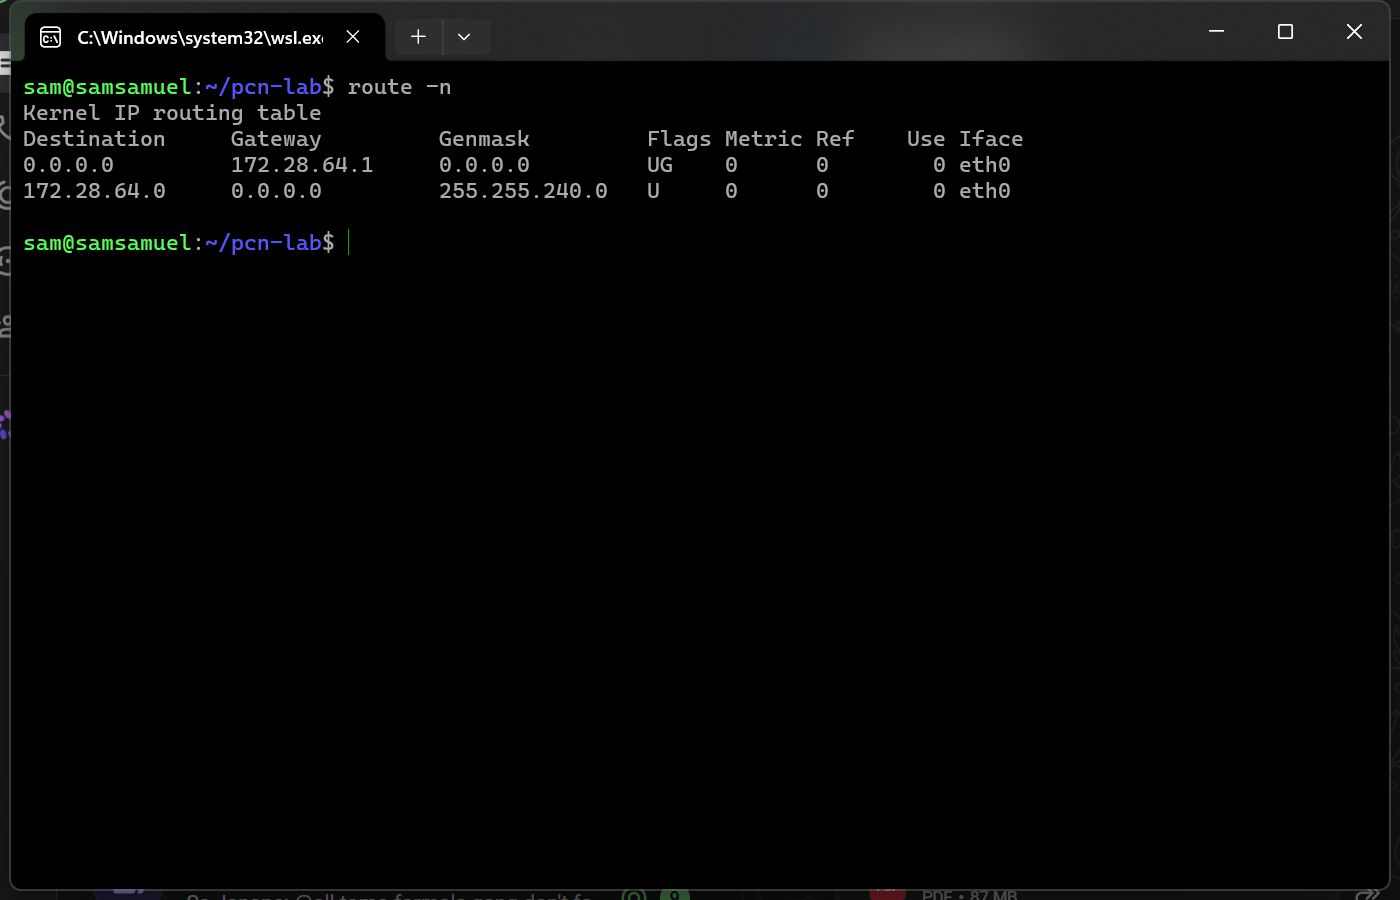
\includegraphics[width=0.85\linewidth]{ss/05_route.png}
\caption{route -n -- kernel routing table}
\end{figure}

\textbf{Observation:} Two entries are present: the default route (\texttt{0.0.0.0/0}) via
gateway \texttt{172.28.64.1} on \texttt{eth0} -- this is the WSL2 virtual switch on the
Windows host, and every packet not destined for the local subnet leaves through it -- and a
directly-connected route for \texttt{172.28.64.0/255.255.240.0}, the local subnet reachable
without a gateway. This matches the addressing seen in \texttt{ifconfig} exactly, and the
gateway address is the same first hop later reported by \texttt{traceroute}.

%===================================================================
\subsection{nmap}
\textbf{Purpose:} Network exploration and security-auditing tool; probes a target's TCP/UDP
ports to determine which are open, and with \texttt{-sV} attempts to fingerprint the service
and version listening on each open port.\\
\textbf{Command used:} \texttt{nmap -sV -T4 -p 22,80,443,9929,31337 scanme.nmap.org}\\
\textit{Target note: \texttt{scanme.nmap.org} is the Nmap Project's own public test host,
explicitly provided for learners to scan; no other host was targeted, in line with
responsible/authorised scanning practice.}

\begin{figure}[H]
\centering
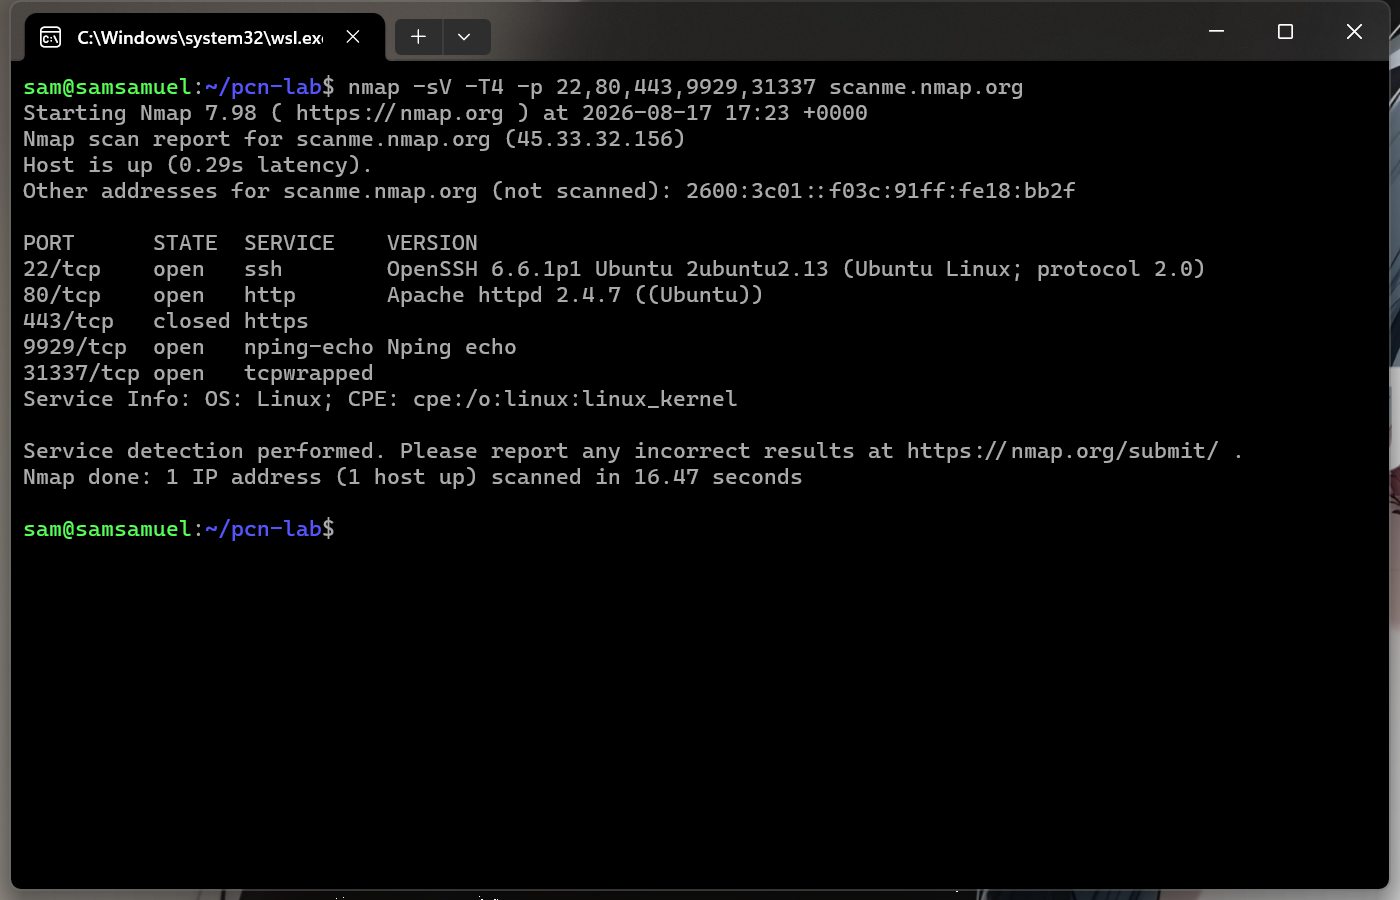
\includegraphics[width=0.85\linewidth]{ss/06_nmap.png}
\caption{nmap -sV version-detection scan against scanme.nmap.org}
\end{figure}

\textbf{Observation:} Of the five ports probed, \texttt{22/tcp} is open running
\texttt{OpenSSH 6.6.1p1} on Ubuntu, \texttt{80/tcp} is open running \texttt{Apache
httpd 2.4.7}, \texttt{443/tcp} is closed (no HTTPS listener), and \texttt{9929/tcp} /
\texttt{31337/tcp} are open running \texttt{nping-echo} and a \texttt{tcpwrapped} service
respectively -- these last two are Nmap's own deliberately-exposed test ports on that host.
Nmap also fingerprinted the OS as Linux from the TCP/IP stack behaviour. Version detection
(\texttt{-sV}) took about 16 seconds for 5 ports, since it goes beyond a plain SYN scan to
send protocol-specific probes and match responses against its signature database.

%===================================================================
\subsection{tcpdump}
\textbf{Purpose:} Captures and prints packets crossing a network interface in real time,
matching an optional filter expression (here, ICMP traffic on \texttt{eth0}) -- the
command-line equivalent of what Assignment 4 uses Wireshark's GUI for.\\
\textbf{Command used:} \texttt{tcpdump -i eth0 -nn -c 5 icmp} (run as root, since raw packet
capture needs \texttt{CAP\_NET\_RAW}), with a \texttt{ping} run concurrently in the same
shell to generate ICMP traffic for it to capture.

\begin{figure}[H]
\centering
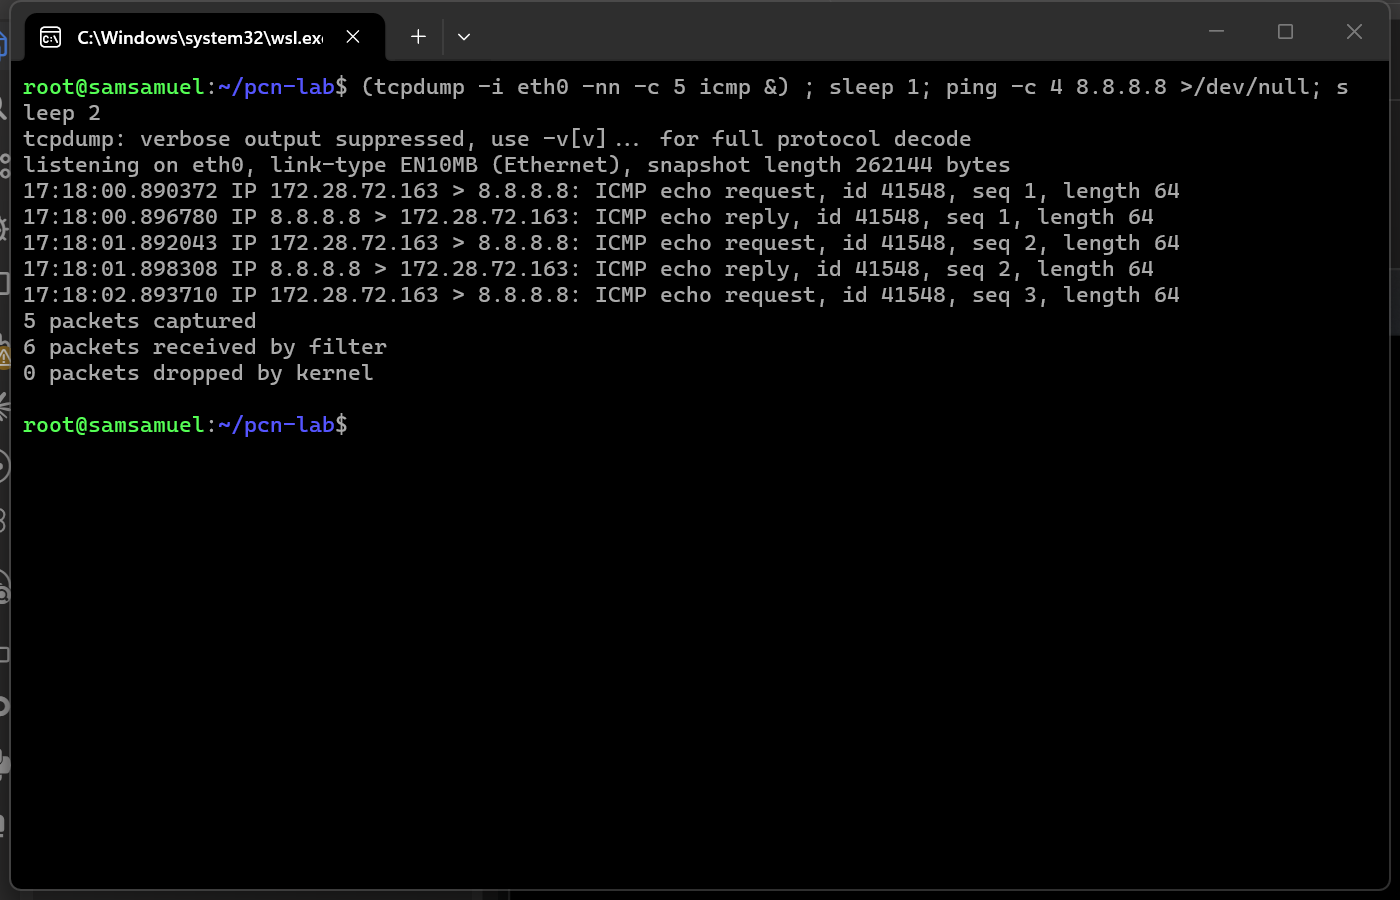
\includegraphics[width=0.85\linewidth]{ss/07_tcpdump.png}
\caption{tcpdump capturing ICMP echo request/reply pairs generated by a concurrent ping}
\end{figure}

\textbf{Observation:} tcpdump captured the ICMP echo request/reply pairs between this host
(\texttt{172.28.72.163}) and \texttt{8.8.8.8} with microsecond-resolution timestamps,
sequence numbers and payload length -- exactly the same exchange \texttt{ping} summarised in
Section~2.4, but now visible packet-by-packet at the network layer instead of as a
round-trip-time summary. This is the same technique Wireshark uses under the hood
(\texttt{tcpdump} and Wireshark both sit on \texttt{libpcap}); \texttt{tcpdump} is the
capture engine without the GUI.

%===================================================================
\subsection{dig}
\textbf{Purpose:} Performs a DNS lookup and prints the full query/response, including the
resource records, query time, and which DNS server answered -- more detailed than
\texttt{nslookup}.\\
\textbf{Command used:} \texttt{dig google.com}

\begin{figure}[H]
\centering
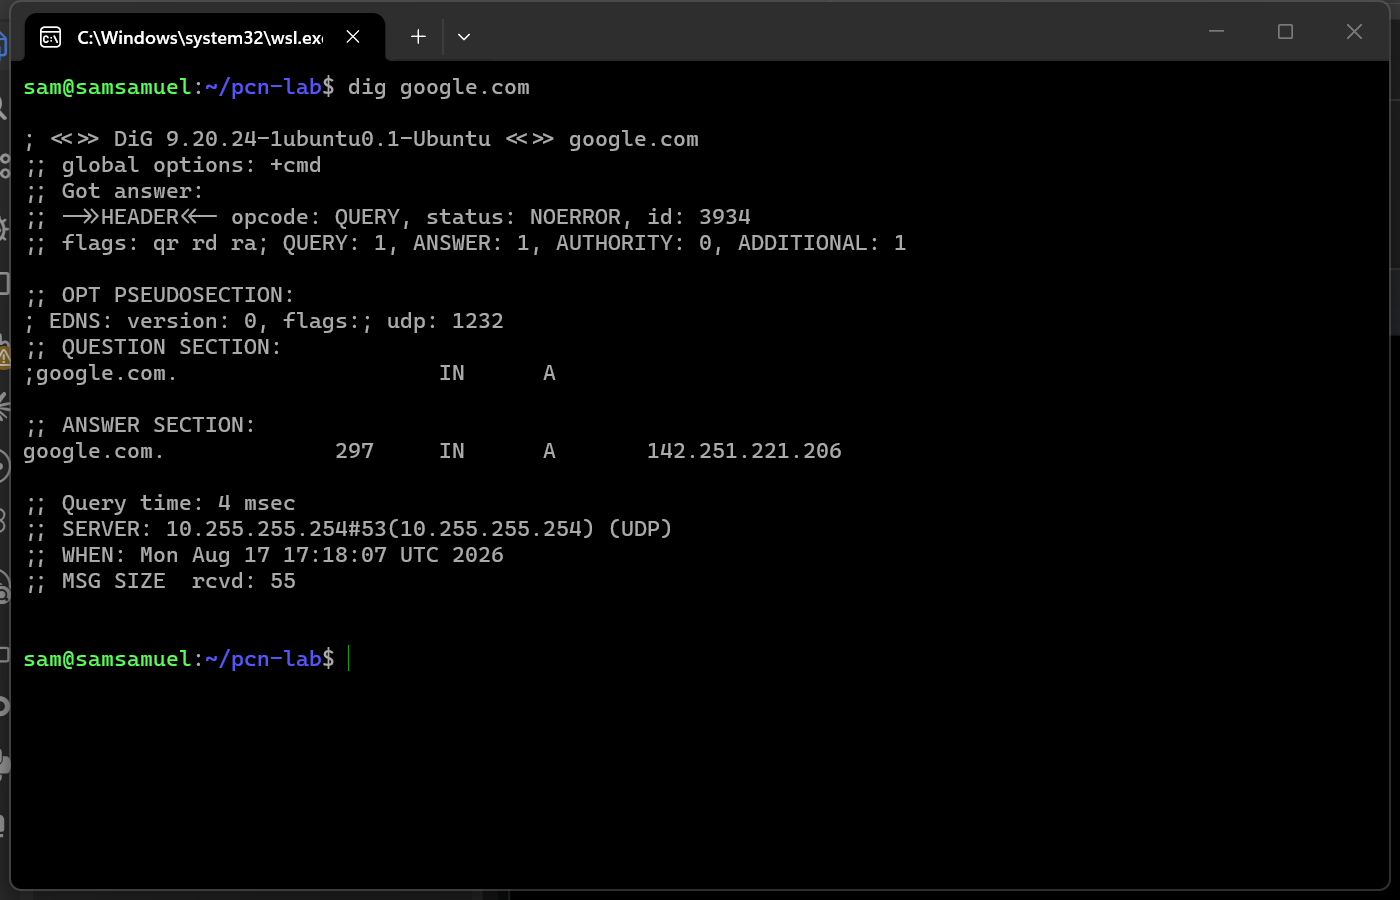
\includegraphics[width=0.85\linewidth]{ss/08_dig.png}
\caption{dig google.com}
\end{figure}

\textbf{Observation:} The query resolved \texttt{google.com} to \texttt{142.251.221.206} in
4\,ms, answered by \texttt{10.255.255.254:53} -- WSL's internal DNS stub, which itself
forwards to the Windows host's configured resolver. The header shows
\texttt{flags: qr rd ra} (response, recursion desired, recursion available) and a single
\texttt{ANSWER} record, confirming the query used UDP (the default transport for DNS,
falling back to TCP only for large/truncated responses).

%===================================================================
\subsection{traceroute}
\textbf{Purpose:} Maps the sequence of routers (hops) a packet passes through to reach a
destination, by sending probes with increasing TTL and recording which router returns the
``TTL exceeded'' ICMP error at each hop.\\
\textbf{Command used:} \texttt{traceroute -m 15 8.8.8.8}

\begin{figure}[H]
\centering
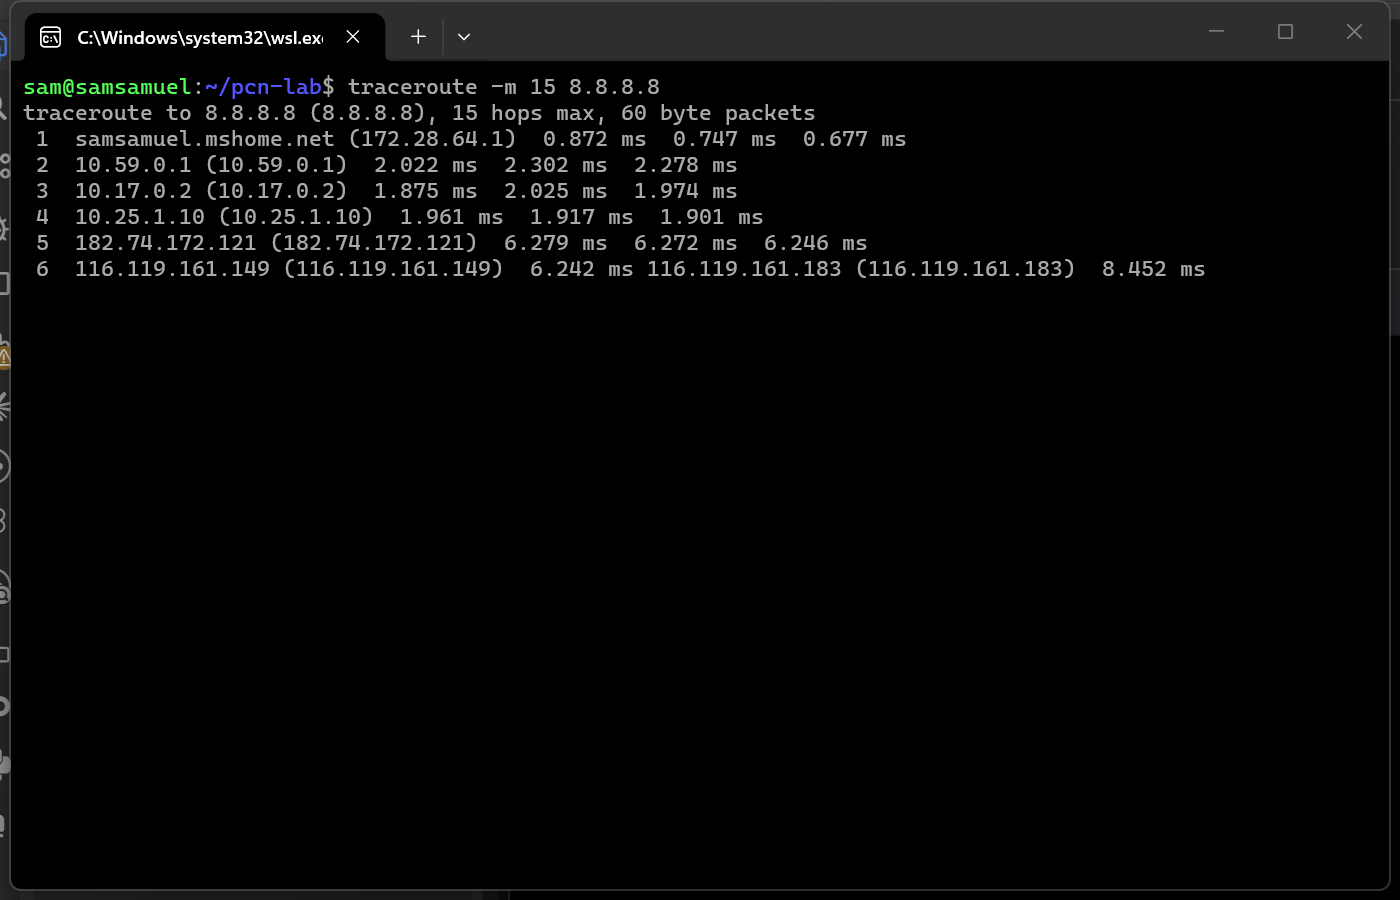
\includegraphics[width=0.85\linewidth]{ss/09_traceroute.png}
\caption{traceroute -m 15 8.8.8.8}
\end{figure}

\textbf{Observation:} The first hop, \texttt{samsamuel.mshome.net (172.28.64.1)}, is the
WSL2/Hyper-V virtual gateway on the Windows host itself -- matching the default-route
gateway seen in Section~2.5. From there the path crosses a couple of private-range hops
(likely the ISP's internal network / CGNAT) before reaching public IP space and, by hop 6,
Google's network, where multiple addresses answering the same hop indicate ECMP (the ISP is
load-balancing across parallel links to Google's edge). Total latency to a hop close to
Google was under 10\,ms, consistent with the low RTT seen from \texttt{ping}.

%===================================================================
\subsection{mtr}
\textbf{Purpose:} Combines \texttt{ping} and \texttt{traceroute} into one continuously-updating
tool -- it traces the path like traceroute but keeps sending probes to every hop, giving a
live per-hop loss/latency statistics table instead of a single traceroute snapshot.\\
\textbf{Command used:} \texttt{mtr -rw -c 5 8.8.8.8} (\texttt{-r} report mode / non-interactive,
\texttt{-c 5} five probe cycles)

\begin{figure}[H]
\centering
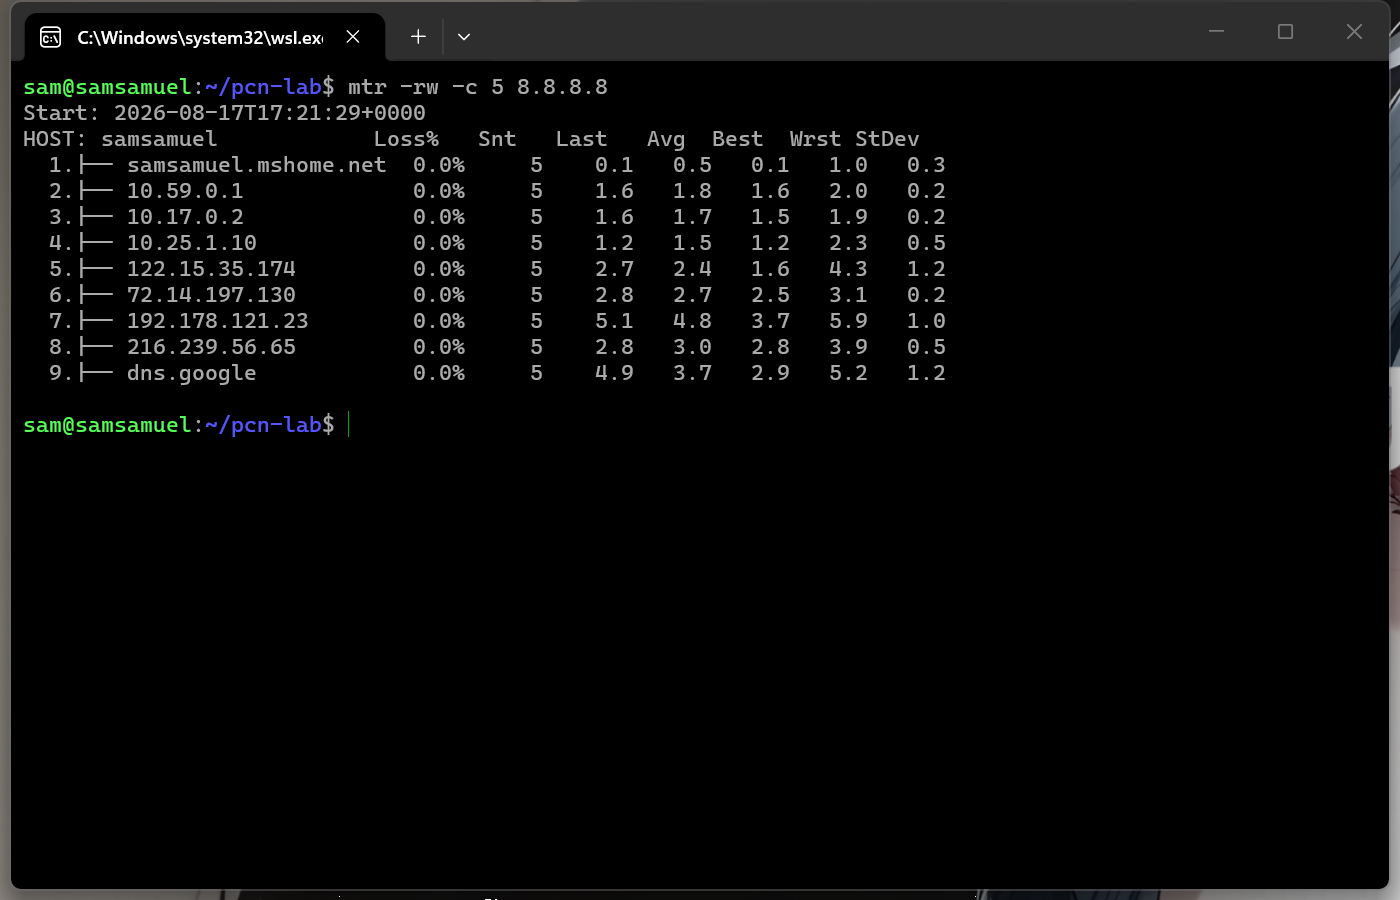
\includegraphics[width=0.85\linewidth]{ss/10_mtr.png}
\caption{mtr -rw -c 5 8.8.8.8 -- report mode}
\end{figure}

\textbf{Observation:} Across all 9 hops and 5 probe cycles each, loss stayed at
\texttt{0.0\%} on every hop, and the \texttt{Avg}/\texttt{Best}/\texttt{Worst}/\texttt{StDev}
columns show latency growing gradually with hop count, with the largest jump between the
local gateway and the ISP core (hop 5, \texttt{122.15.35.174}) -- the point where traffic
leaves the WSL/home network and enters the wider internet. The final hop resolves via
reverse DNS to \texttt{dns.google}, confirming the destination is indeed one of Google's
public DNS front-ends.

%===================================================================
\subsection{curl}
\textbf{Purpose:} Command-line tool for transferring data with a URL, supporting HTTP(S),
FTP and many other protocols; \texttt{-v} prints the full request/response including the
TLS handshake.\\
\textbf{Command used:} \texttt{curl -v https://example.com -o /dev/null}

\begin{figure}[H]
\centering
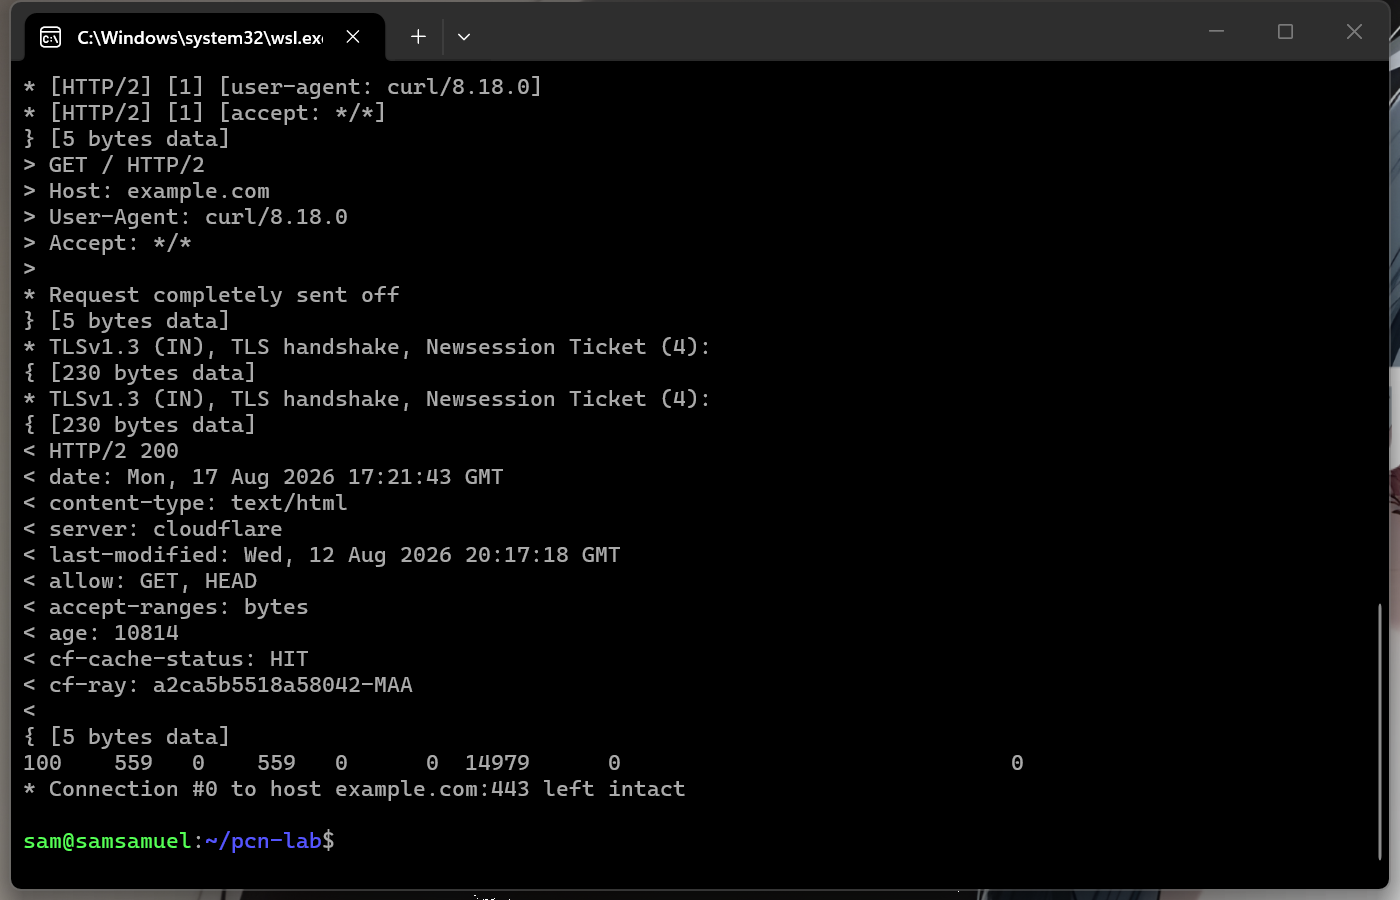
\includegraphics[width=0.85\linewidth]{ss/11_curl.png}
\caption{curl -v https://example.com -- verbose TLS handshake and HTTP/2 response}
\end{figure}

\textbf{Observation:} curl resolved \texttt{example.com} to a Cloudflare-hosted address
(\texttt{104.20.23.154}), completed a \texttt{TLSv1.3} handshake (client hello, server hello,
certificate, finished), negotiated \texttt{HTTP/2} over ALPN, and received a
\texttt{200} response served from Cloudflare's edge cache
(\texttt{cf-cache-status: HIT}). This single command demonstrates the full modern HTTPS
stack -- TCP connect, TLS 1.3 key exchange and certificate verification, then an HTTP/2
request/response -- that Assignment 3's C client will have to build manually at the socket
level for its basic HTTP case.

%===================================================================
\subsection{wget}
\textbf{Purpose:} Non-interactive command-line downloader, commonly used to fetch a file or
whole page from an HTTP(S)/FTP URL and save it to disk.\\
\textbf{Command used:} \texttt{wget https://example.com -O example\_wget.html}

\begin{figure}[H]
\centering
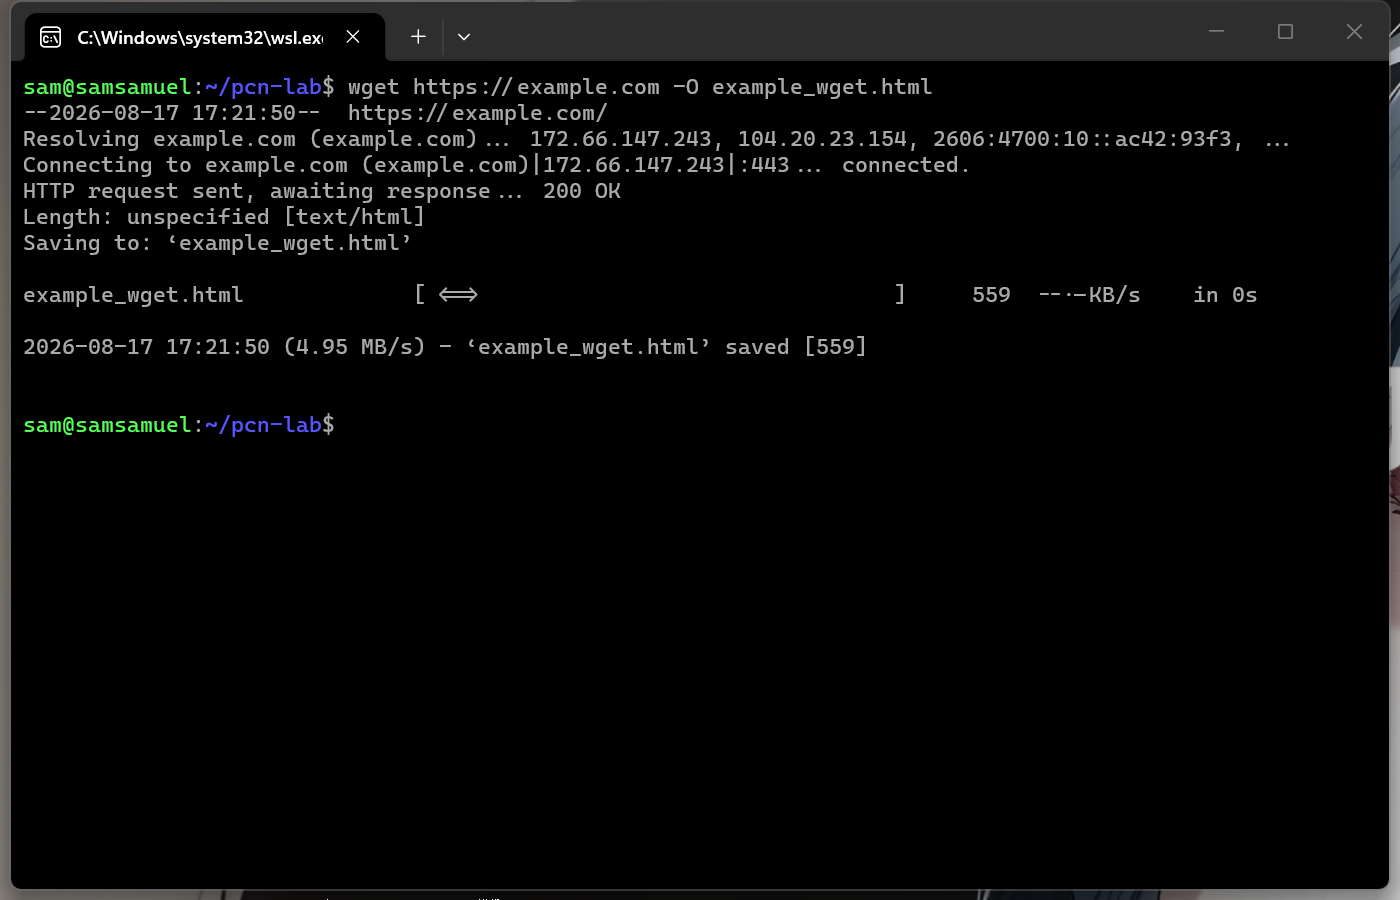
\includegraphics[width=0.85\linewidth]{ss/12_wget.png}
\caption{wget saving example.com to a local file}
\end{figure}

\textbf{Observation:} wget resolved and connected to the same Cloudflare address as curl,
received a \texttt{200 OK} with \texttt{Content-Type: text/html}, and saved the 559-byte
response body to \texttt{example\_wget.html} on disk -- unlike \texttt{curl}, which by
default streams to stdout, \texttt{wget}'s whole design centres on saving the retrieved
resource to a file, which is exactly the behaviour Assignment 3's HTTP client needs to
replicate for downloading \texttt{index.html} / \texttt{sample.pdf} / \texttt{image.jpg}.

%===================================================================
\subsection{tracepath}
\textbf{Purpose:} A traceroute-like tool that does not require root privileges (unlike
classic \texttt{traceroute}), and additionally reports the discovered Path MTU.\\
\textbf{Command used:} \texttt{tracepath 8.8.8.8}

\begin{figure}[H]
\centering
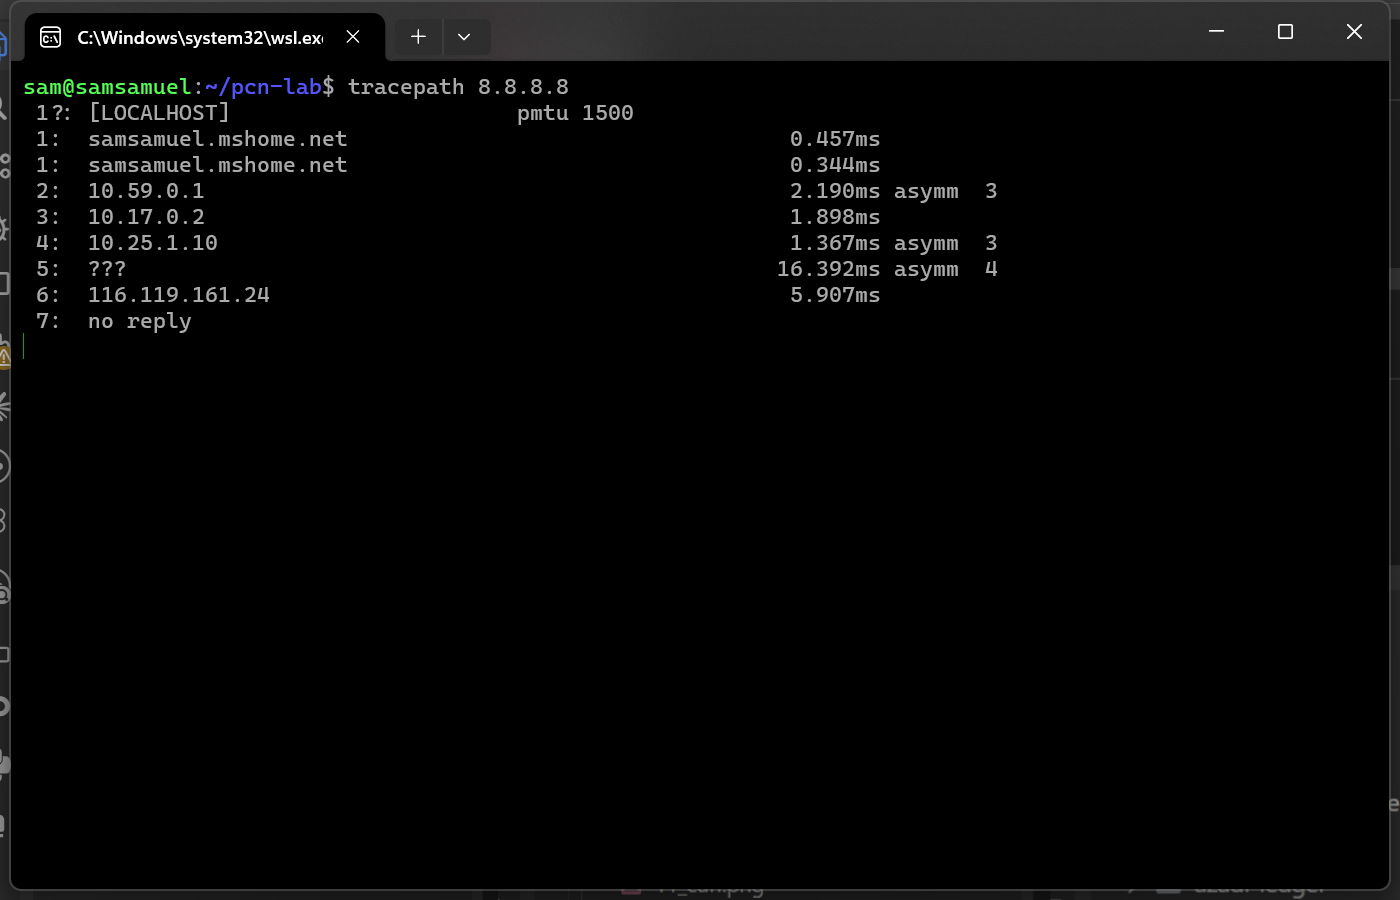
\includegraphics[width=0.85\linewidth]{ss/13_tracepath.png}
\caption{tracepath 8.8.8.8}
\end{figure}

\textbf{Observation:} tracepath discovered a Path MTU of 1500 bytes (the Ethernet standard,
confirming no tunnelling/fragmentation is reducing the effective packet size along the
path), and traced 6 responding hops with asymmetric round-trip marks (\texttt{asymm}) on a
couple of hops -- meaning the reverse path taken by the ICMP reply does not mirror the
forward path exactly, which is common on the modern, multi-path internet. The final
\texttt{no reply} at hop 7 is expected: many routers close to the destination rate-limit or
drop the low-TTL UDP probes tracepath uses, without that indicating an actual fault.

%===================================================================
\subsection{nslookup}
\textbf{Purpose:} Interactive/batch tool to query DNS servers for a name's resource
records -- the older, simpler counterpart to \texttt{dig}.\\
\textbf{Command used:} \texttt{nslookup google.com}

\begin{figure}[H]
\centering
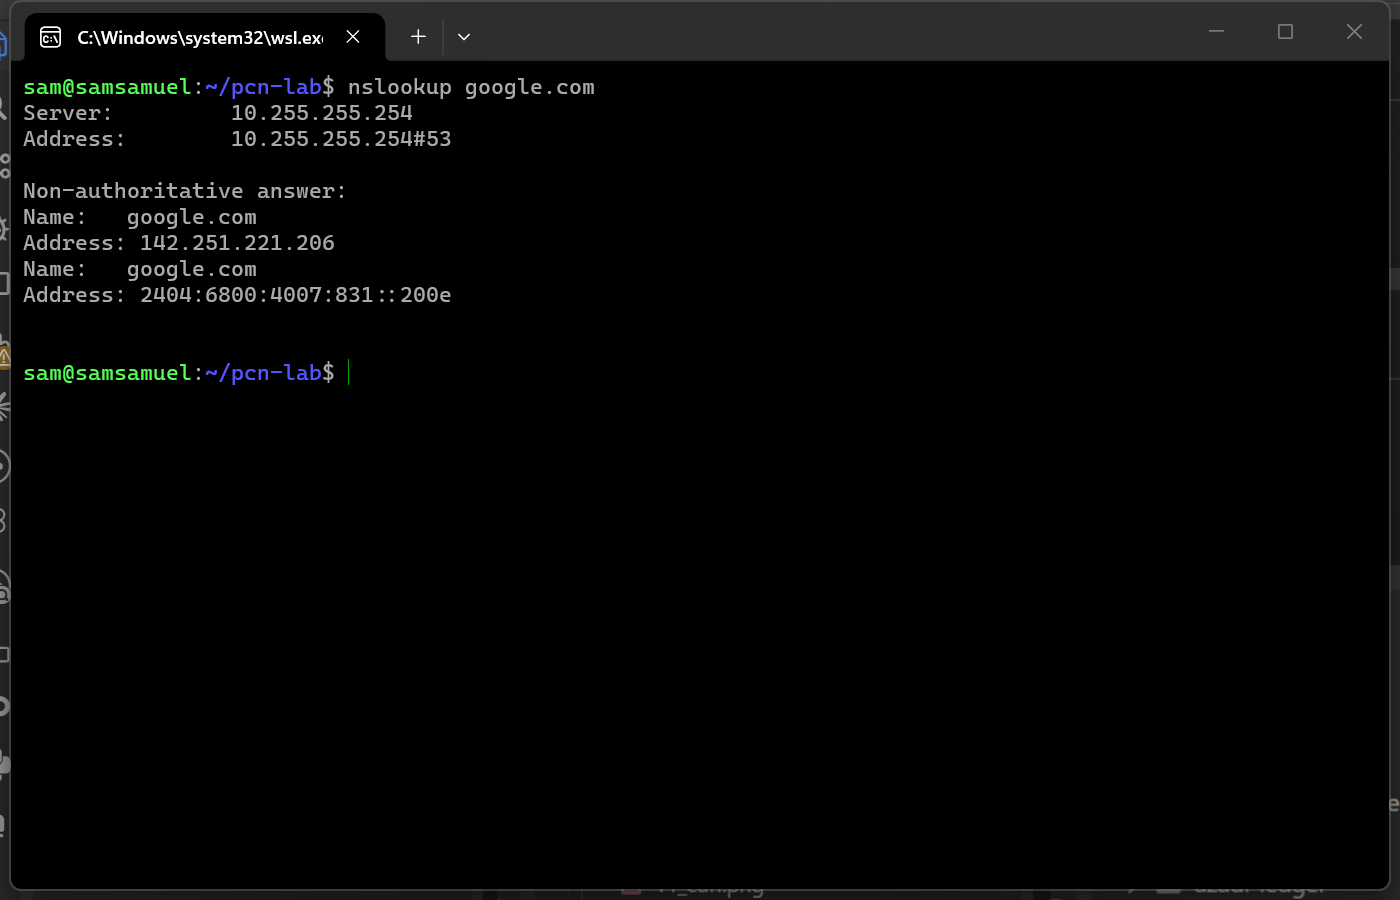
\includegraphics[width=0.85\linewidth]{ss/14_nslookup.png}
\caption{nslookup google.com}
\end{figure}

\textbf{Observation:} The resolver at \texttt{10.255.255.254} returned both an IPv4
(\texttt{142.251.221.206}) and an IPv6 (\texttt{2404:6800:4007:831::200e}) address for
\texttt{google.com} under \texttt{Non-authoritative answer} -- meaning the answer came from
the resolver's cache/forwarding rather than directly from Google's authoritative
nameservers, which is the normal, expected mode for an everyday DNS lookup.

%===================================================================
\subsection{host}
\textbf{Purpose:} A concise DNS lookup utility, well suited to scripting, that by default
prints A, AAAA and MX records in one line each.\\
\textbf{Command used:} \texttt{host google.com}

\begin{figure}[H]
\centering
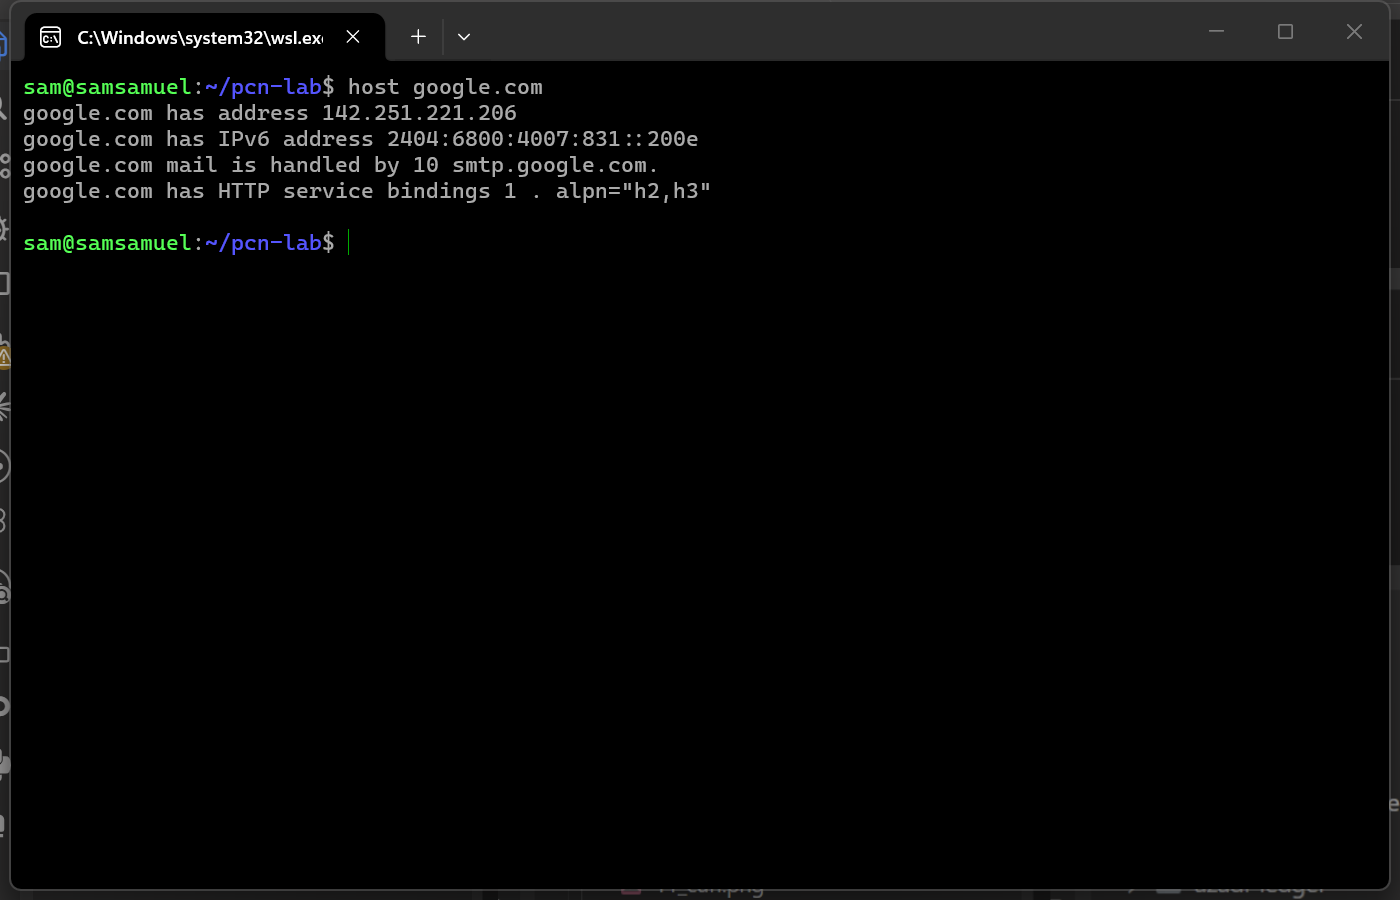
\includegraphics[width=0.85\linewidth]{ss/15_host.png}
\caption{host google.com}
\end{figure}

\textbf{Observation:} In one compact query, \texttt{host} listed google.com's A record
(\texttt{142.251.221.206}), AAAA record, mail-exchanger record
(\texttt{10 smtp.google.com}), and an \texttt{HTTPS} service-binding record advertising
ALPN support for \texttt{h2} and \texttt{h3} (HTTP/2 and HTTP/3) -- the same underlying data
as \texttt{dig}/\texttt{nslookup}, just formatted for quick reading rather than full protocol
detail.

%===================================================================
\subsection{whois}
\textbf{Purpose:} Queries domain (or IP) registry databases for registration
information -- registrar, registration/expiry dates, nameservers and domain status.\\
\textbf{Command used:} \texttt{whois google.com}

\begin{figure}[H]
\centering
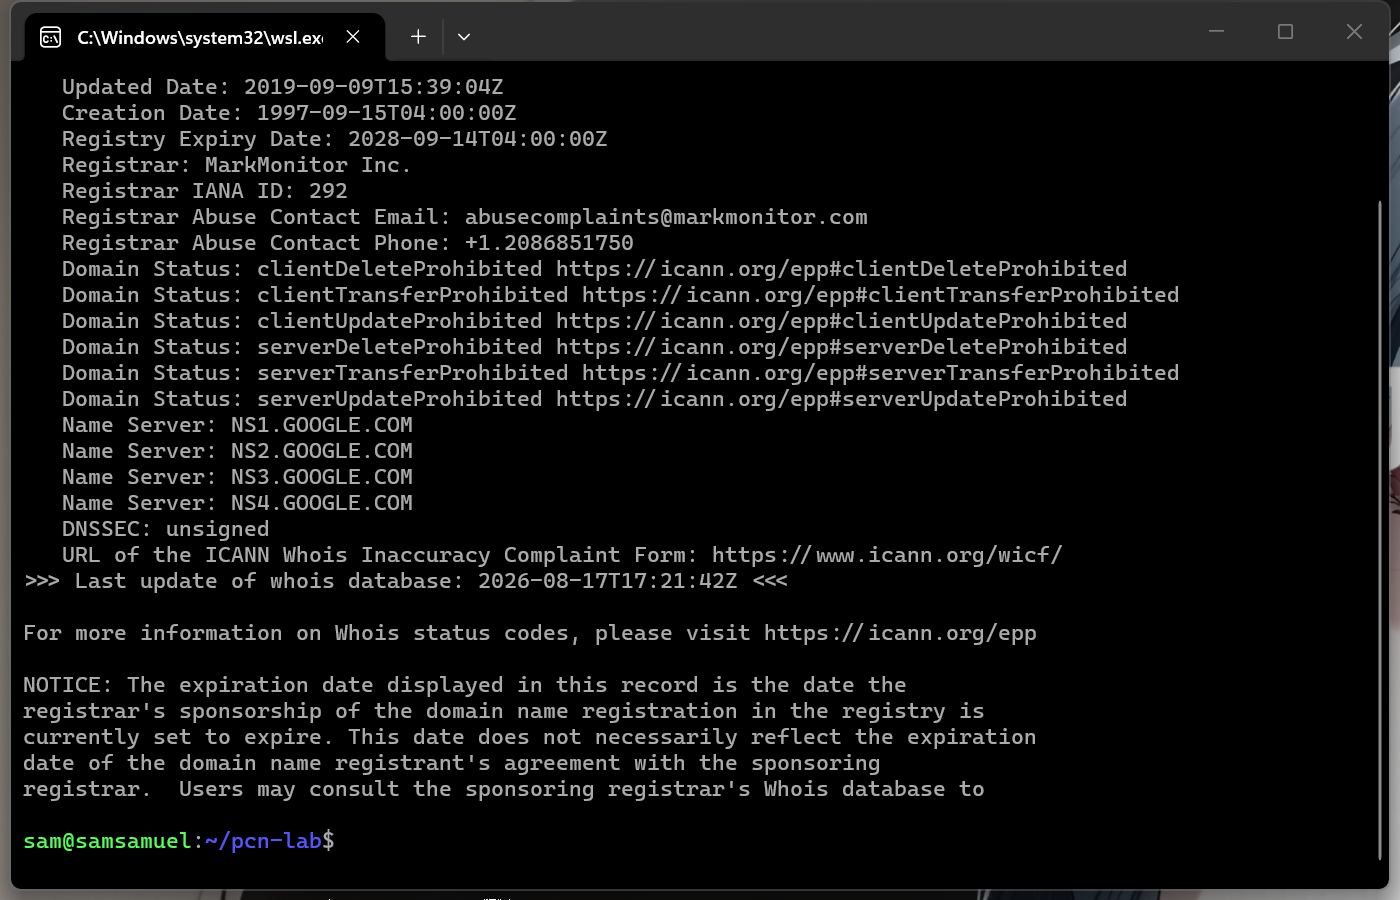
\includegraphics[width=0.85\linewidth]{ss/16_whois.png}
\caption{whois google.com}
\end{figure}

\textbf{Observation:} \texttt{google.com} is registered through \textbf{MarkMonitor Inc.},
created \textbf{1997-09-15} and set to expire \textbf{2028-09-14}, delegated to
\texttt{NS1--NS4.GOOGLE.COM}. The domain status flags
(\texttt{clientTransferProhibited}, \texttt{clientDeleteProhibited}, etc.) show it is locked
against unauthorised transfer/deletion -- standard practice for a high-value domain. Unlike
the DNS tools above, \texttt{whois} queries the registry/registrar database directly rather
than the DNS resolution chain, so it answers ``who owns this name'' rather than ``what
address does this name point to''.

\clearpage
\section{Part B --- Socket Programming System Calls}

The table below summarises the purpose, key parameters and return value of each system
call, grouped by role in the client--server lifecycle. \texttt{TCP/IP and UDP} applications
in the last column note where a call is mandatory (M), optional/common (O), or not
applicable (--) for each transport.

\subsection{Socket creation, addressing and lifecycle}

\begin{longtable}{|p{2.6cm}|p{6.6cm}|p{2cm}|p{3.6cm}|}
\hline
\textbf{Call} & \textbf{Purpose \& key parameters} & \textbf{Returns} & \textbf{TCP / UDP use} \\ \hline
\endhead

\texttt{socket()} &
\texttt{int socket(int domain, int type, int protocol)} creates an endpoint for
communication. \texttt{domain=AF\_INET} selects IPv4; \texttt{type} is
\texttt{SOCK\_STREAM} for TCP or \texttt{SOCK\_DGRAM} for UDP; \texttt{protocol=0} lets the
kernel pick the default for that type. &
New socket file descriptor, or $-1$ on error. &
M (both) -- first call in every socket program. \\ \hline

\texttt{bind()} &
\texttt{int bind(int sockfd, const struct sockaddr *addr, socklen\_t addrlen)} associates a
socket with a local IP address and port, described by a \texttt{struct sockaddr\_in}
(\texttt{sin\_family}, \texttt{sin\_port}, \texttt{sin\_addr}). &
$0$ on success, $-1$ on error. &
M for servers (both); optional for clients (kernel auto-assigns an ephemeral port
otherwise). \\ \hline

\texttt{listen()} &
\texttt{int listen(int sockfd, int backlog)} marks a \texttt{SOCK\_STREAM} socket as
passive/listening and sets \texttt{backlog}, the maximum length of the queue of pending
(not-yet-accepted) connections. &
$0$ on success, $-1$ on error. &
M (TCP server only) -- meaningless for UDP, which is connectionless. \\ \hline

\texttt{connect()} &
\texttt{int connect(int sockfd, const struct sockaddr *addr, socklen\_t addrlen)}. For TCP,
performs the three-way handshake with the given peer. For UDP, it merely records a default
peer address so subsequent \texttt{send()}/\texttt{recv()} can be used instead of
\texttt{sendto()}/\texttt{recvfrom()} -- no packets are exchanged. &
$0$ on success, $-1$ on error. &
M (TCP client); O (UDP client, to fix the peer). \\ \hline

\texttt{accept()} &
\texttt{int accept(int sockfd, struct sockaddr *addr, socklen\_t *addrlen)} blocks until a
connection is pending on a listening socket, then returns a \emph{new} socket descriptor
dedicated to that one client; \texttt{addr} is filled with the client's address. &
New connected-socket descriptor, or $-1$ on error. &
M (TCP server only). \\ \hline

\texttt{close()} &
\texttt{int close(int fd)} releases the file descriptor; for TCP this initiates connection
teardown (FIN) once all references to the socket are closed. &
$0$ on success, $-1$ on error. &
M (both) -- every socket opened must eventually be closed. \\ \hline

\end{longtable}

\subsection{Buffers and byte order}

\begin{longtable}{|p{2.6cm}|p{6.6cm}|p{2cm}|p{3.6cm}|}
\hline
\textbf{Call} & \textbf{Purpose \& key parameters} & \textbf{Returns} & \textbf{TCP / UDP use} \\ \hline
\endhead

\texttt{bzero()} &
\texttt{void bzero(void *s, size\_t n)} fills \texttt{n} bytes at \texttt{s} with zero;
routinely used to clear a \texttt{struct sockaddr\_in} before filling in its fields, so
padding bytes don't contain garbage. &
None (void). &
O (both) -- good practice before populating an address struct. \\ \hline

\texttt{htons()} &
\texttt{uint16\_t htons(uint16\_t hostshort)} converts a 16-bit value (typically a port
number) from host byte order to network (big-endian) byte order. &
The value in network byte order. &
M (both) -- every \texttt{sin\_port} assignment. \\ \hline

\texttt{htonl()} &
\texttt{uint32\_t htonl(uint32\_t hostlong)} -- the 32-bit equivalent of \texttt{htons()},
used for IP addresses (e.g. \texttt{INADDR\_ANY}) held as a 32-bit integer. &
The value in network byte order. &
O (both) -- needed whenever an address is built numerically rather than via
\texttt{inet\_pton}. \\ \hline

\texttt{ntohs()} &
\texttt{uint16\_t ntohs(uint16\_t netshort)} converts a 16-bit value from network byte order
back to host byte order -- the inverse of \texttt{htons()}; used when reading a port back
out of a received \texttt{sockaddr\_in} to print/compare it. &
The value in host byte order. &
O (both) -- e.g. printing a peer's port from \texttt{getpeername()}. \\ \hline

\texttt{ntohl()} &
\texttt{uint32\_t ntohl(uint32\_t netlong)} -- the 32-bit inverse of \texttt{htonl()}. &
The value in host byte order. &
O (both). \\ \hline

\end{longtable}

\subsection{Data transfer}

\begin{longtable}{|p{2.6cm}|p{6.6cm}|p{2cm}|p{3.6cm}|}
\hline
\textbf{Call} & \textbf{Purpose \& key parameters} & \textbf{Returns} & \textbf{TCP / UDP use} \\ \hline
\endhead

\texttt{read()} &
\texttt{ssize\_t read(int fd, void *buf, size\_t count)} -- generic POSIX I/O call; on a
connected socket it behaves like \texttt{recv(fd, buf, count, 0)}. &
Bytes read ($\ge 0$), $0$ on EOF/peer closed, $-1$ on error. &
O (TCP, connected sockets). \\ \hline

\texttt{write()} &
\texttt{ssize\_t write(int fd, const void *buf, size\_t count)} -- generic POSIX I/O call;
on a connected socket behaves like \texttt{send(fd, buf, count, 0)}. &
Bytes written, or $-1$ on error. &
O (TCP, connected sockets). \\ \hline

\texttt{send()} &
\texttt{ssize\_t send(int sockfd, const void *buf, size\_t len, int flags)} -- sends data on
a \emph{connected} socket (TCP, or UDP after \texttt{connect()}); \texttt{flags} such as
\texttt{MSG\_DONTWAIT} modify behaviour. &
Bytes sent, or $-1$ on error. &
M (TCP); O (connected UDP). \\ \hline

\texttt{recv()} &
\texttt{ssize\_t recv(int sockfd, void *buf, size\_t len, int flags)} -- receives data on a
connected socket. &
Bytes received, $0$ if peer closed, $-1$ on error. &
M (TCP); O (connected UDP). \\ \hline

\texttt{sendto()} &
\texttt{ssize\_t sendto(int sockfd, const void *buf, size\_t len, int flags, const struct
sockaddr *dest\_addr, socklen\_t addrlen)} -- sends a datagram to an explicit destination
without requiring \texttt{connect()} first (\texttt{dest\_addr=NULL} on an already-connected
socket falls back to plain \texttt{send()} behaviour). &
Bytes sent, or $-1$ on error. &
M (UDP, connectionless); O (TCP). \\ \hline

\texttt{recvfrom()} &
\texttt{ssize\_t recvfrom(int sockfd, void *buf, size\_t len, int flags, struct sockaddr
*src\_addr, socklen\_t *addrlen)} -- receives a datagram and records who it came from in
\texttt{src\_addr}. &
Bytes received, or $-1$ on error. &
M (UDP, connectionless); O (TCP). \\ \hline

\end{longtable}

\subsection{Multiplexing, configuration and name resolution}

\begin{longtable}{|p{2.6cm}|p{6.6cm}|p{2cm}|p{3.6cm}|}
\hline
\textbf{Call} & \textbf{Purpose \& key parameters} & \textbf{Returns} & \textbf{TCP / UDP use} \\ \hline
\endhead

\texttt{select()} &
\texttt{int select(int nfds, fd\_set *readfds, fd\_set *writefds, fd\_set *exceptfds,
struct timeval *timeout)} -- blocks (up to \texttt{timeout}) until one of the given file
descriptors is ready for I/O; the classic way to wait on several sockets, or to add a
timeout to a blocking \texttt{accept()}/\texttt{recv()}. &
Number of ready descriptors, $0$ on timeout, $-1$ on error. &
O (both) -- essential for a single-threaded server handling multiple clients (Assignment 2
uses \texttt{pthread} instead). \\ \hline

\texttt{setsockopt()} &
\texttt{int setsockopt(int sockfd, int level, int optname, const void *optval, socklen\_t
optlen)} -- sets a socket option, e.g. \texttt{SOL\_SOCKET}/\texttt{SO\_REUSEADDR} to allow
immediately rebinding a port still in \texttt{TIME\_WAIT}. &
$0$ on success, $-1$ on error. &
O (both) -- almost always used on the listening/bound socket of a server. \\ \hline

\texttt{fcntl()} &
\texttt{int fcntl(int fd, int cmd, ...)} -- general file-descriptor control;
\texttt{F\_GETFL}/\texttt{F\_SETFL} read/modify flags such as \texttt{O\_NONBLOCK}, commonly
used to switch a socket to non-blocking mode. &
Depends on \texttt{cmd} (e.g. current flags for \texttt{F\_GETFL}), $-1$ on error. &
O (both). \\ \hline

\texttt{getpeername()} &
\texttt{int getpeername(int sockfd, struct sockaddr *addr, socklen\_t *addrlen)} -- returns
the address of the peer connected to \texttt{sockfd}, useful for logging/authorising a
client after \texttt{accept()}. &
$0$ on success, $-1$ on error. &
O (TCP, connected sockets). \\ \hline

\texttt{gethostname()} &
\texttt{int gethostname(char *name, size\_t len)} -- returns the local machine's hostname. &
$0$ on success, $-1$ on error. &
O (both) -- informational/logging use. \\ \hline

\texttt{gethostbyname()} &
\texttt{struct hostent *gethostbyname(const char *name)} -- resolves a hostname to one or
more IP addresses (\texttt{h\_addr\_list}); the classic (now legacy, superseded by
\texttt{getaddrinfo()}) way for a client to turn a server name into an address before
\texttt{connect()}. &
Pointer to a \texttt{struct hostent}, or \texttt{NULL} on failure. &
O (both) -- client-side name resolution. \\ \hline

\texttt{gethostbyaddr()} &
\texttt{struct hostent *gethostbyaddr(const void *addr, socklen\_t len, int type)} --
reverse DNS: resolves an IP address back to a hostname (a PTR lookup), the inverse of
\texttt{gethostbyname()}. &
Pointer to a \texttt{struct hostent}, or \texttt{NULL} if no PTR record. &
O (both) -- e.g. a server logging the resolved name of a connecting client. \\ \hline

\end{longtable}

\subsection{Empirical demonstration}

To confirm the calls above actually behave as described rather than only on paper, a small
TCP client/server pair was written in C (\texttt{as1/src/server.c},
\texttt{as1/src/client.c}) that genuinely exercises all 23 calls from the two tables: the
server creates, configures, binds and listens on a socket; \texttt{select()} waits for a
connection; \texttt{accept()} takes it; \texttt{fcntl()}, \texttt{getpeername()} and
\texttt{gethostbyaddr()} inspect the new connection; and three request/reply turns are
exchanged, one turn each over \texttt{recv()}/\texttt{send()},
\texttt{recvfrom()}/\texttt{sendto()} and \texttt{read()}/\texttt{write()}, so every
data-transfer call is genuinely used at least once, not just described. Rather than
hard-coding a demo string, both programs read each message from \texttt{stdin} (via
\texttt{fgets}) exactly as a person typing at the keyboard would -- the excerpt below is the
server side's message loop:

\begin{lstlisting}[caption={Excerpt of as1/src/server.c -- interactive message loop}]
bzero(inbuf, sizeof(inbuf));
recv(connfd, inbuf, sizeof(inbuf) - 1, 0);
strip_newline(inbuf);
printf("them: %s\n", inbuf);
printf("you: ");
fflush(stdout);
fgets(outbuf, sizeof(outbuf), stdin);
strip_newline(outbuf);
printf("%s\n", outbuf);
send(connfd, outbuf, strlen(outbuf), 0);
\end{lstlisting}

Two terminals were run side by side: one where the server was compiled and started
(\texttt{gcc -Wall -o server server.c \&\& ./server}), and a second, separate terminal where
the client was compiled and connected to it
(\texttt{gcc -Wall -o client client.c \&\& ./client 127.0.0.1}) once the server was already
listening.

\begin{figure}[H]
\centering
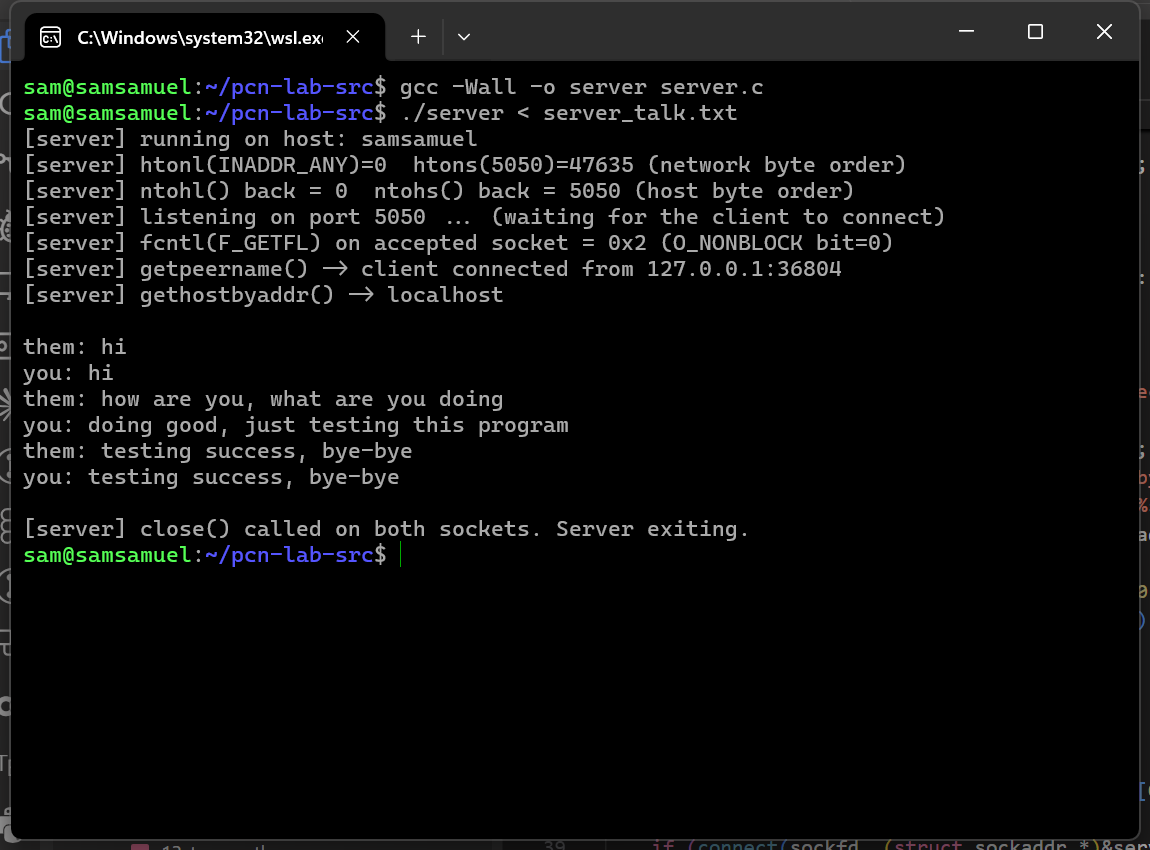
\includegraphics[width=0.85\linewidth]{ss/17a_server_terminal.png}
\caption{Server terminal -- compiles, binds/listens, accepts the connection, and exchanges
three messages}
\end{figure}

\begin{figure}[H]
\centering
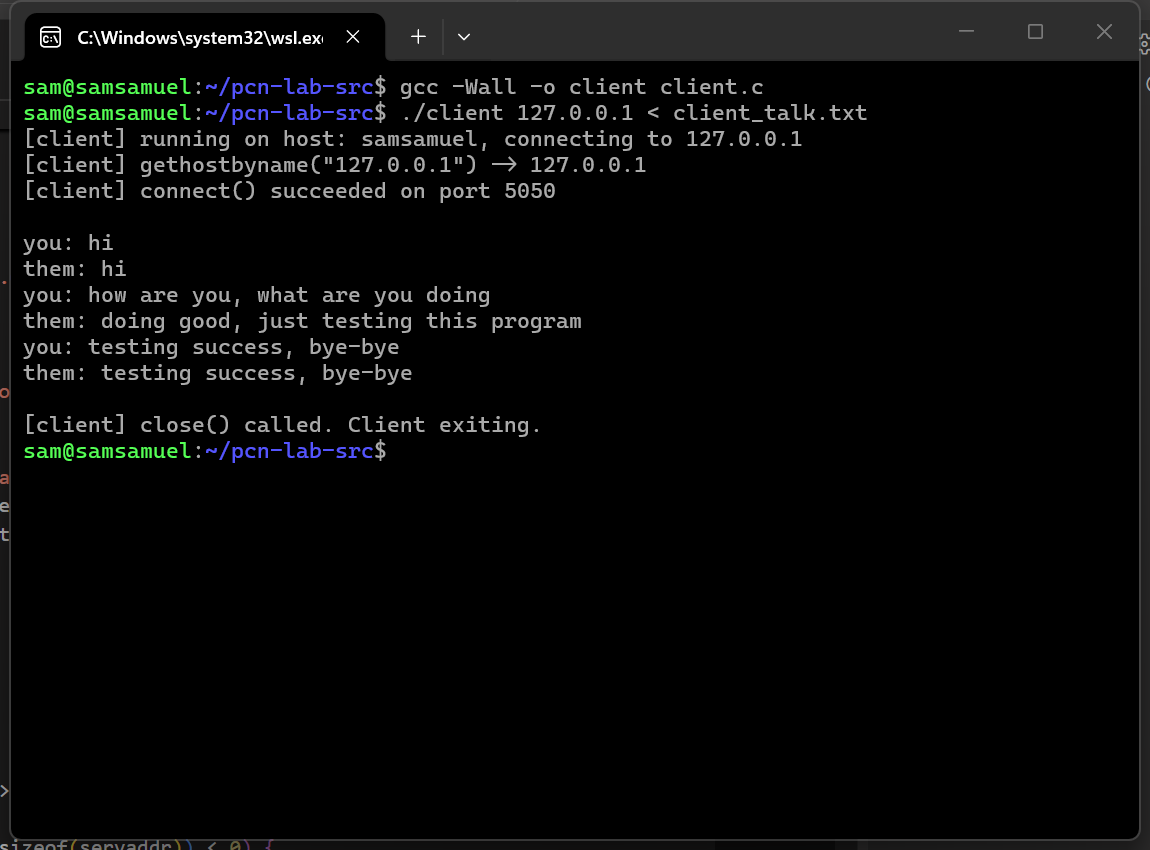
\includegraphics[width=0.85\linewidth]{ss/17b_client_terminal.png}
\caption{Client terminal -- compiles, connects, and exchanges the same three messages}
\end{figure}

\textbf{Observation:} The byte-order conversions are visible directly in the output --
\texttt{htons(5050)} prints as \texttt{47635}, which is exactly 5050 with its two bytes
swapped ($5050 = \texttt{0x13BA}$, swapped to $\texttt{0xBA13} = 47635$), and
\texttt{ntohs()} converts it straight back to \texttt{5050}, confirming the two functions
are true inverses on this little-endian host. \texttt{getpeername()} correctly reported the
client's loopback address and ephemeral source port; \texttt{gethostbyaddr()} resolved
\texttt{127.0.0.1} back to \texttt{localhost}; and \texttt{fcntl(F\_GETFL)} showed the
accepted socket's \texttt{O\_NONBLOCK} bit as \texttt{0}, i.e. still blocking, since it was
never switched into non-blocking mode. Both terminals show an identical three-line
conversation, confirming the byte stream sent by one side's \texttt{send()}/
\texttt{sendto()}/\texttt{write()} was received intact by the other side's
\texttt{recv()}/\texttt{recvfrom()}/\texttt{read()} in the same order it was sent -- the
in-order, reliable delivery guarantee that TCP provides and that Assignment 2's UDP path
will not.

\clearpage
\section{Learning Outcome}
\begin{itemize}
\item Learned how to use everyday Linux networking commands (\texttt{netstat},
\texttt{ifconfig}, \texttt{ping}, \texttt{route}, \texttt{nmap}, \texttt{tcpdump},
\texttt{dig}, \texttt{traceroute}, \texttt{mtr}, \texttt{curl}, \texttt{wget},
\texttt{tracepath}, \texttt{nslookup}, \texttt{host}, \texttt{whois}) to check a machine's
network status, routing, and connectivity, and to read/interpret their output.
\item Understood what each socket system call (\texttt{socket}, \texttt{bind},
\texttt{listen}, \texttt{accept}, \texttt{connect}, \texttt{send}/\texttt{recv},
\texttt{sendto}/\texttt{recvfrom}, \texttt{select}, etc.) actually does, instead of just
knowing their names.
\item Got hands-on practice writing and running a real TCP client-server program in C, and
saw byte-order conversion (\texttt{htons}/\texttt{ntohs}) and data delivery work correctly
across two live terminals.
\end{itemize}

\end{document}
